\documentclass[11pt,letterpaper]{article}

% Use the custom AA279D template style
\usepackage{AA279D_template}
\usepackage{hyperref, gensymb, amsmath}

% User inputs: change as needed for each assignment
\newcommand{\workingDate}{\textsc{2018 $|$ April $|$ 16}}
\newcommand{\userName}{Yutao Liu}
\newcommand{\institution}{Stanford University}
\newcommand{\theTitle}{AA 279D}

\begin{document}
\title{279}
% Set up the title page
\begin{titlepage}
    \begin{center}
        \vspace*{1cm}
        
        \Huge
        \textbf{TanDEM-X/TerraSAR-X Constellation: Formation Flying in LEO}
        
        \vspace{0.5cm}
        \LARGE
        \ 
        
        \vspace{1.00cm}
        \textbf{\userName}
        \vspace{1.00cm}
        
        \vfill
        \begin{figure}[H]
		\centering 
		\includegraphics[width = 5.5in]{Figures/tt.jpg}
		\label{Figure: Title Graphic}
		\end{figure}
        \        
        
        \Large
        AA 279D - Spacecraft Formation-Flying and Rendezvous\\
        Stanford University\\
        
    \end{center}
\end{titlepage}

% Update the revision history with each assignment
\section*{Revision History}

\begin{table}[ht]
\centering
\caption{Summary of project revisions.}
\begin{tabular}{ll}
\toprule
\textbf{Rev} & \textbf{Changes} \\
\hline
PS1 & \tabitem Created document \\
    & \tabitem Added problem set 1 material  \\
\hline
PS2 & \tabitem Added problem set 2 material  \\
    & \tabitem Example revision statement 1  \\
    & \tabitem Example revision statement 2  \\
\hline
PS3 & \tabitem Added problem set 3 material  \\
\bottomrule
\end{tabular}
\label{table:revision history}

\end{table}

\newpage
\tableofcontents

\newpage
\section{Preliminary mission study}
\subsection{Mission description}
The TanDEM-X spacecraft launched on 21 June 2010 complements the existing TerraSAR-X satellite to form the first configurable SAR (Synthetic Aperture Radar) interferometer with baselines of a few hundred meters in space. The primary goal of the TanDEM-X (TerraSAR-X add-on for Digital Elevation Measurement) mission is to generate a global digital elevation model (DEM). 

The satellites will fly in formation and operate in parallel for three years to cover the entire surface of Earth. Together, the  identical spacecrafts orbit Earth in a polar dusk-dawn orbit with a 515 km altitude and an 11 day repeat period. Besides controlling the TerraSAR-X spacecraft to fly in a predefined tube of 250 m radius, regular control maneuvers will be exercised to maintain a specific formation geometry in each mission phase.\cite{montenbruck}

A schematic representation of the satellites as well as their operating conditions can be found below.
\begin{figure}[H]
	\centering
    \includegraphics[height=3in]{Figures/tandem.jpg}
    \caption{The TerraSAR-X and TanDEM-X satellites are nearly identical in construction.}
    \label{figure:Sats}
\end{figure}

\begin{table}[ht]
\centering
\caption{Satellite specifications}
\label{my-label}
\begin{tabular}{ll}
\toprule
Orbit altitude       & 514 km \\
Orbit inclination    & 97.4\degree   \\
Satellite mass       & 1330 kg \\
Satellite dimensions &                \\
Height               & 5 m       \\
Diameter             & 2.4 m    \\
\bottomrule
\end{tabular}
\end{table}

The up-to-date orbital elements of the constellation could be retrieved from \href{www.heavens-above.com}{heavens-above.com}:
\begin{table}[ht]
\centering
\caption{Current orbital elements}
\label{my-label}
\begin{tabular}{lll}
\toprule
\textbf{Orbital Element	}		   & \textbf{TerraSAR-X}   & \textbf{TanDEM-X}      \\
\hline
Epoch (UTC):                       & 16 April 2018 04:07:14 & 16 April 2018 07:16:58 \\ 
Eccentricity:                      & 0.0002035              &.0002293                \\ 
Inclination:                       & 97.4464\degree         & 97.4452\degree \\
Perigee height:                    & 507 km                 & 507 km\\
Apogee height:                     & 510 km                 & 510 km\\
Right ascension of ascending node: & 114.6359\degree        & 114.5018\degree \\
Argument of perigee:               & 72.8528\degree         & 77.4517\degree \\
Revolutions per day:               & 15.19142245            & 15.19144898 \\
Mean anomaly at epoch:             & 344.5982\degree        & 339.8946\degree \\
Orbit number at epoch:             & 43363                  & 60087 \\
\bottomrule
\end{tabular}
\end{table}

\subsection{Mission Orbit Simulation}
The first step in the mission study would be to simulate the trajectory of TerraSAR-X, which was launched 15 June 2007, 02:14 UTC into a polar,  sun-synchronous dusk-dawn orbit at 514km altitude. This forms an ellipse of 6886.39 km semi-major axis and 0.0001445 eccentricity at an inclination of 97.44\degree.

\begin{figure}[H]
	\centering
    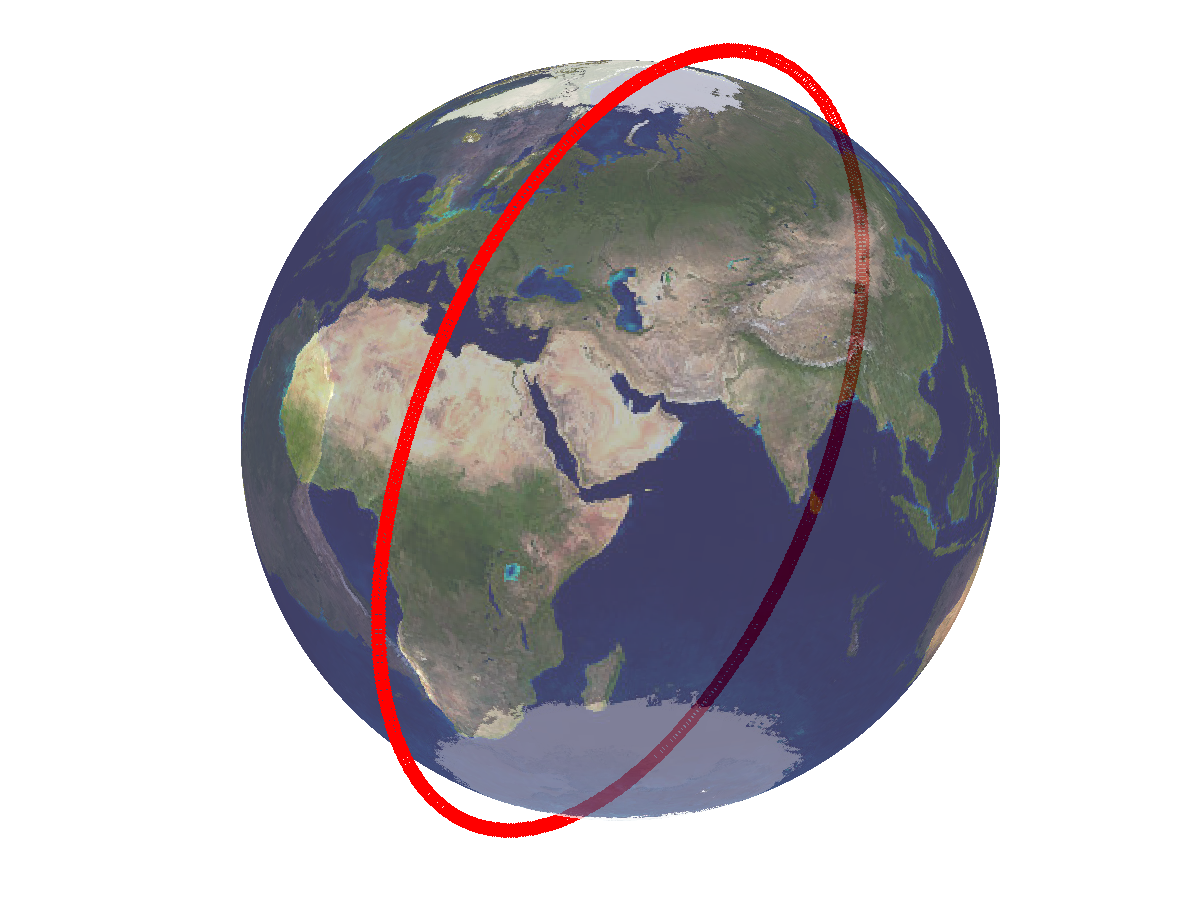
\includegraphics[height=3in]{Figures/Traj.eps}
    \caption{Osculating orbit of TerraSAR-X}
    \label{figure:traj}
\end{figure}
\subsubsection{Effects of $J_2$ perturbation}
% Equation \ref{Equation: golden rule} is demonstrating the use of custom commands embedded in the .sty sheet which can simplify your main LaTeX document.
% \begin{align}
% 	\VEL{N}{A_0} &= \DIFF{N}{ \POS{N_0}{A_0} } = \VEL{R}{A_0} + \OMEGA{N}{R} \times \POS{N_0}{A_0}
% 	\label{Equation: golden rule}
% \end{align}
% where $\VEL{N}{A_0}$ is the velocity of point $A_0$ in reference frame $\FRAME{N}$, $\VEL{R}{A_0}$ is the velocity of $A_0$ in reference frame $\FRAME{R}$, $\OMEGA{N}{R}$ is the angular velocity of $\FRAME{R}$ in $\FRAME{N}$, and $\POS{N_0}{A_0}$ is the position vector from point $N_0$ (which is fixed in $\FRAME{N}$) to $A_0$.\\

% Absolute value: $\abs{-5} = 5$.\\
% Vector norm: $\norm{\vec{r}} = \sqrt{r_X^2 + r_Y^2 + r_Z^2}$\\



\section{Relative motion study}

\begin{figure}[H]
	\centering
    \includegraphics[height=3in]{Figures/monobi.jpeg}
    \caption{Concept of TanDEM-X InSAR observations in bistatic (left) and monostatic (right) modes}
    \label{figure:modes}
\end{figure}

\begin{figure}[H]
	\centering
    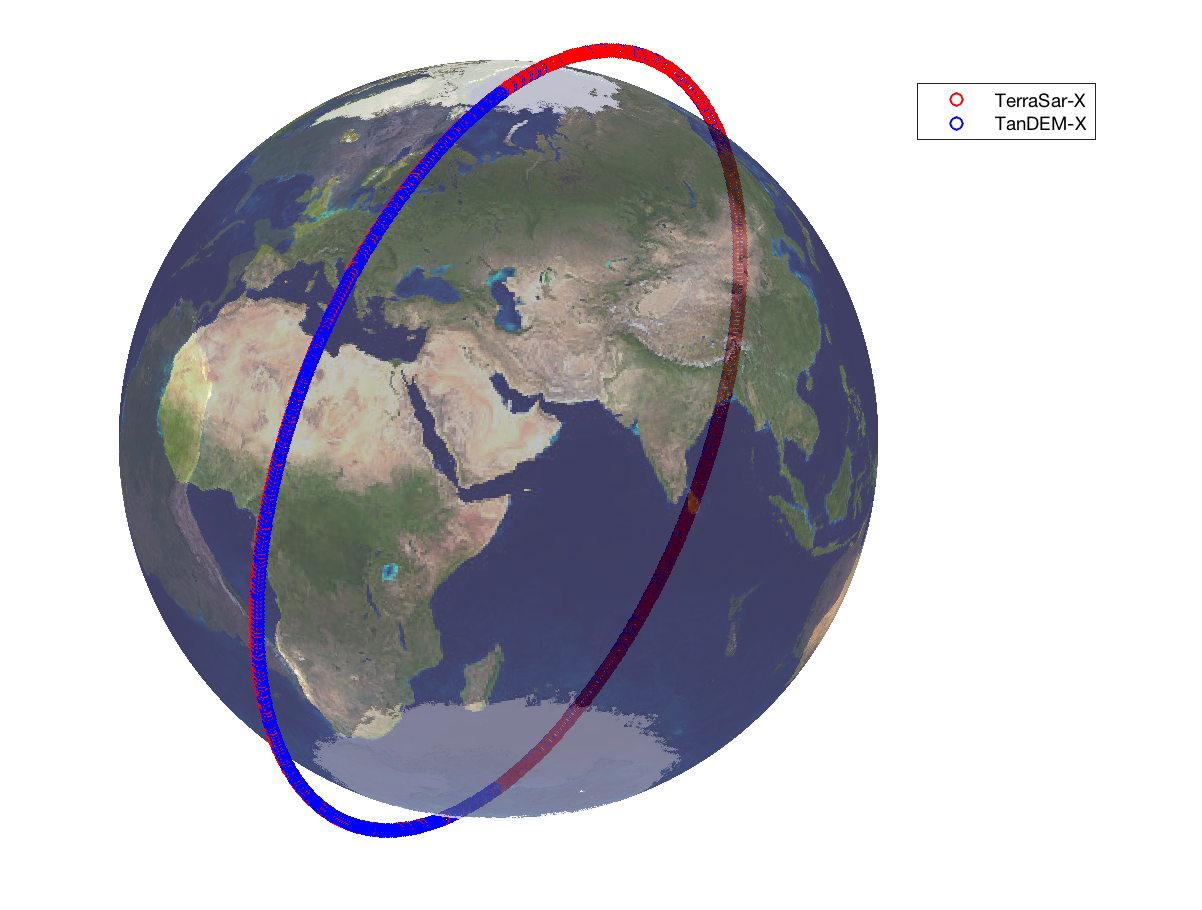
\includegraphics[height=3in]{Figures/Traj2.eps}
    \caption{Simulation of TerraSAR-X and TanDEM-X trajectories}
    \label{figure:traj}
\end{figure}



% % \documentclass[11pt,letterpaper]{article}

% % Use the custom AA279D template style
% \usepackage{AA279D_template}
% \usepackage{hyperref, gensymb, amsmath}
% \begin{document}

$$^\mathbb{I}{\delta\mathbf{v}_L} = ^\mathbb{I}{\mathbf{R}}^\mathcal{L}$$
orbit design usually done in mean space $\langle\cdot\rangle$

osculating oe as a transformation from mean
$\textbf{\oe}(\langle\textbf{\oe}\rangle)$

use Newton-Raphson to compute $\langle\Delta\textbf{\oe}\rangle$ iterative update until error condition

$$\ddot{\mathbf{\rho}} = 
\mathbf{f}
(\mathbf{\rho}, \dot{\mathbf{\rho}}, \mathbf{r}_0, \dot{\mathbf{r}}_0, \mathbf{\theta}_0, \dot{\mathbf{\theta}}_0,)
$$
when $e_0=0$ this becomes $\ddot{\mathbf{\rho}} = 
\mathbf{g}(\mathbf{\rho}, \dot{\mathbf{\rho}}, \mathbf{\theta}_0,)$

when will the deputy appear stationary to the chief?

\[
	\begin{cases}
    	(x+a_0)^2 + y^2 = a_0^2\\z=0
    \end{cases}
\]

when $\rho/r_0 <<1$ the HOTs drop out to yield a set of linear ODEs
\[
	\begin{cases}
    \begin{aligned}
    	&\ddot{x}-2n_0\dot{y} &-3n^3x &=0\\
        &\ddot{y}+2n_0\dot{x} &       &=0\\
        &\ddot{z}&+n_0^2z             &=0
    \end{aligned}
    \end{cases}
\]

can you replace mean motion of chief with deputy? no longer second order

FF in LEO of small separations can be designed with HCW equations

% \end{document}

%%%%%%%%%%%%%%%%%%%%%%%%%%%%%%%%%%%%%
% References
%%%%%%%%%%%%%%%%%%%%%%%%%%%%%%%%%%%%%
\newpage
\begin{thebibliography}{9}
\bibitem{alfriend}K. Alfriend, S. Vadali, P. Gurfil, J. How, and L. Breger, \textit{Spacecraft Formation Flying: Dynamics, Control, and Navigation}. Elsevier Astrodynamics Series, 2010. 

% https://onlinelibrary.wiley.com/doi/epdf/10.1002/j.2161-4296.2011.tb02587.x
\bibitem{montenbruck}O. Montenbruck, M. Wermuth, and R. Kahle,
\textit{GPS Based Relative Navigation for the TanDEM-X Mission - First Flight Results}. DLR/GSOC, September 2010.

% http://elib.dlr.de/63481/1/Damico_PhD_01022010.pdf
\bibitem{damico}S. D'Amico, \textit{Autonomous Formation Flying
in Low Earth Orbit}. PhD Thesis. TU Delft, 2010.

% 

\end{thebibliography}
\addcontentsline{toc}{section}{References}

\end{document}